\documentclass{minimal}
\usepackage{tikz}
\usetikzlibrary{calc,matrix}

\begin{document}
  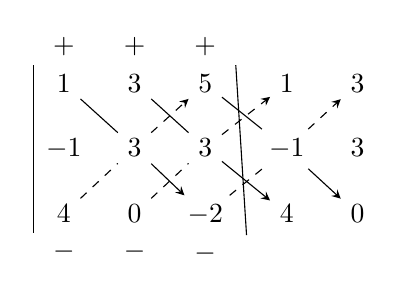
\begin{tikzpicture}[>=stealth]
    \matrix [%
      matrix of math nodes,
      column sep=1em,
      row sep=1em
    ] (sarrus) {%
      1 & 3 & 5 & 1 & 3 \\
      -1 & 3 & 3 & -1 & 3 \\
      4 & 0 & -2 & 4 & 0 \\
    };

    \path ($(sarrus-1-1.north west)-(0.5em,0)$) edge ($(sarrus-3-1.south west)-(0.5em,0)$)
          ($(sarrus-1-3.north east)+(0.5em,0)$) edge ($(sarrus-3-3.south east)+(0.5em,0)$)
          (sarrus-1-1)                          edge            (sarrus-2-2)
          (sarrus-2-2)                          edge[->]        (sarrus-3-3)
          (sarrus-1-2)                          edge            (sarrus-2-3)
          (sarrus-2-3)                          edge[->]        (sarrus-3-4)
          (sarrus-1-3)                          edge            (sarrus-2-4)
          (sarrus-2-4)                          edge[->]        (sarrus-3-5)
          (sarrus-3-1)                          edge[dashed]    (sarrus-2-2)
          (sarrus-2-2)                          edge[->,dashed] (sarrus-1-3)
          (sarrus-3-2)                          edge[dashed]    (sarrus-2-3)
          (sarrus-2-3)                          edge[->,dashed] (sarrus-1-4)
          (sarrus-3-3)                          edge[dashed]    (sarrus-2-4)
          (sarrus-2-4)                          edge[->,dashed] (sarrus-1-5);

    \foreach \c in {1,2,3} {\node[anchor=south] at (sarrus-1-\c.north) {$+$};};
    \foreach \c in {1,2,3} {\node[anchor=north] at (sarrus-3-\c.south) {$-$};};
  \end{tikzpicture}
\end{document}
